\subsection*{Abstract}

Formal specifications are necessary to guarantee software meets critical safety
properties, but retrofitting specifications to existing software requires
considerable resources and expertise. Although inference eases discovery of
specifications, existing inference techniques are limited in targeting different
specification conditions. Particularly, inference of postconditions has rarely
been the targeted focus of prior investigations. This paper presents a static
program analysis that automatically synthesizes postconditions from pure program
syntax. These postconditions represent final values of variables in numerical
loops. For each variable, the analysis finds one approximative postcondition, of
at most polynomial form, if it is expressible in the underlying theory. This
theory is a sound and compositional flow calculus with complexity-theoretic
origins. However, applying the flow calculus to postcondition inference required
several enhancements. As technical contributions, we resolve multiple open
problems about the flow calculus and increase its expressive power. Experiments
and comparison study show the postcondition analysis is orthogonal to
alternative techniques and generalizes to classic algorithms. These findings
suggest the postcondition analysis can offer support in specification tasks even
if full implementation details are still in flux.

\subsection{Introduction}
\label{sec:pc-intro}

Software engineers have an aphorism that warns against publishing releases on
Fridays. It is shared lightheartedly, but embeds serious commentary about the
normalcy of software instability. Formal methods provides the techniques to
improve and achieve rigorous software quality guarantees. Unfortunately,
integrating formal methods to mainstream software development workflows remains
challenging due to, \eg lack of training and tool-specific
issues~\cite{beek2024}. Continued research effort must be dedicated to reducing
the entry barriers.

This paper aims to improve accessibility of formal methods.
We do this by introducing a program analysis that synthesizes partial specification conditions.
We develop an automatic inference of approximative postconditions in numerical loops.
Postconditions are specialized assertions that must hold after the loop terminates.
They are complementary to {inductive loop invariants}, \ie conditions that must hold pre-iteration and be preserved by the loop~\cite{sankaranarayanan2004}.
Although postconditions may be derivable from invariants, loop invariant inference is one of the hardest problems in verification~\cite{dillig2013,si2018}.
Therefore, we suggest the opposite approach: starting with postconditions.
It is well-known that having postconditions supports discovery of inductive invariants~\cite{furia2010}.
Moreover, as generalized assertions, postconditions assist in various software development activities~\cite{nguyen2022}, like testing~\cite{alagarsamy2024,zhang2015} and code maintenance~\cite{rosenblum1995}.
However, dedicated studies of postcondition inference are a novelty in research literature~\cite{popeea2006,molina2021}.

Specifications must be precise, consistent, and complete descriptions of program behavior.
Making formal specifications mechanically verifiable requires they are expressed in a structured language.
However, defining formal specifications is non-trivial and requires expertise.
In the meantime, various resource analyses~\cite{jones2009,brockschmidt2016} already compute varied notions of postconditions as means to arrive to their primary result.
Thus, it seems natural that {resource analyses could be used to infer postconditions} for formal specifications.
This is precisely the key intuition we exploit in the paper.
We present a complexity\hyp{}theoretic flow calculus~\cite{jones2009,aubert20222} that we use to automatically infer variable postconditions.
In this view, the program implements the intended behavior, but misses a formal proof.
Our goal is to assist software engineers in completing this missing step.

\subsubsection{Problem formulation and solution overview}
\label{subsec:overview}

We analyze deterministic imperative numerical loops.
The loop may be bounded or unbounded, with unknown termination behavior.
The loop manipulates a fixed number of natural number variables.
Beyond type, we make no assumptions about initial variable values.
Our goal is to automatically infer postconditions of the variables occurring in the loop.
A postcondition is an assertion about a variable's value that holds after iteration, if the loop terminates.
The loop may represent a program {fragment} that is still under development. %, and need not be an executable whole-program.
Reducing contextual information this way is practically motivated because such information is commonly absent in realistic unverified programs.

\autoref{lst:exA} shows a canonical verification problem.
Given a specification with a precondition (\pr|assume|) and a loop command (\pr|for|), the goal of formal verification is to prove that the postcondition (\pr|assert|) is satisfiable.
The program \emph{\explain}, in \autoref{lst:exB}, shows the problem variant we address in the paper.
When precise variable values, precondition, and iteration count are unknown, what postconditions (\qtext) can we infer from the syntax?

\begin{center}
\begin{minipage}{.45\textwidth}
\captionsetup{type=lstlisting}
\begin{center}
\begin{minipage}{.9\textwidth}
\begin{implisting}*[numbers=none,escapeinside=||]
assume(X2|$\leq$|10|$\,\land\,$|X4==2|$\,\land\,$|X5>4);
for(i=0;i<10;i++) {
  X3=X2*X2;
  X3=X3+X5;
  X4=X4+X5; }
assert(X3|$\leq$|100+X5|$\,\land\,$|X4|$\geq$|42);
\end{implisting}
\end{minipage}
\end{center}
\captionof{lstlisting}[Precise context (ideal)]
{Precise context (ideal).}\label{lst:exA}
\end{minipage}\hfill%
\begin{minipage}{.52\textwidth}
\captionsetup{type=lstlisting}
\begin{center}
\begin{minipage}{.85\textwidth}
\begin{implisting}*[numbers=none,escapeinside=||]
for(i=0;i<X1;i++) {
  X3=X2*X2;
  X3=X3+X5;
  X4=X4+X5; }
assert(|\myqm|);
\end{implisting}
\end{minipage}
\end{center}
\captionof{lstlisting}[Imprecise context]
{Imprecise context (ours), \mbox{\explain}.}\label{lst:exB}
\end{minipage}
\end{center}

Our analysis infers postconditions that express the {growth of variable values} in the loop.
Adding postpositions supports discovery of other specification conditions, like invariants,
that then permit formal verification (the Duet analyzer in \autoref{subsec:comparison} is an example).
The analysis is sound, guaranteeing that if a postcondition can be inferred, it is known to hold.

As result, our analysis generates {mwp-bounds}.
These are symbolic expressions describing the value growth of the program variables.
An \emph{mwp-bound}~\cite{jones2009} represent a variable's \emph{final value} in terms of the \emph{initial values} and omitting constants.
An mwp-bound is an approximation of the {upper bound} of the final value.
A critical idea is that the \textbf{mwp-bounds are postconditions}.
Since the problem formulation assumes no pre-conditions, a function in terms of the inputs is the most precise achievable postcondition in most cases.
An mwp-bound is maximally polynomial in form.
A variable value growth that is beyond a polynomial is not expressible as an mwp-bound.
However, our experiments (\autoref{sec:performance}) suggest that this is not a prohibitive limitation.
The analysis successfully assigns postconditions to most variables in a set of diverse benchmarks.

Based on the mwp-bound form, we categorize the variables as linear, iteration-independent, iteration-dependent, or inconclusive (in increasing order).
We discuss the semantics of the categories in~\autoref{subsec:disclaimer};
but briefly, they are behavioral descriptors.
For example, a linear variable has only a light dependency on the containing loop because its value is updated by at most a constant.
While our analysis is not complete for arbitrary programs, we can guarantee that the inferred mwp-bounds are {optimal} (\autoref{subsec:categories}) \wrt in the expressiveness of the flow calculus.
In other words, we find the least upper bound that describes variable value growth.

At program point \qtext, our analysis gives the following result.
\begin{itemize}
\item Variables \pr|X1|, \pr|X2|, and \pr|X5| values have grown at most linearly from the initials
\item Variable  \pr|X3| value is iteration-independent and bounded by \(\max(\prm{X3},\prm{X2}+\prm{X5})\)
\item Variable  \pr|X4| value is iteration-dependent and bounded by \(\prm{X4}+\prm{X1}\times\prm{X5}\)
\end{itemize}

We can determine manually the precise postconditions for comparison.
The linear variables never change from their initial values.
The final value of \pr|X3| is its initial value \pr|X3| or \(\prm{X2}^2+\prm{X5}\), depending on if the loop iterates.
For variable \pr|X4|, the precise postcondition is \(\prm{X4}+\prm{X1}\times\prm{X5}\).

\subsubsection{Contributions}
\label{subsec:contributions}

\begin{enumerate}

\item Our main result is an automatic analysis for postcondition inference in numerical loops (\autoref{sec:analysis}).
The analysis is applicable in imprecise contexts and in absence of initial variable values and program annotations.

\item To obtain the analysis, we extend the flow calculus of mwp-bounds with two new capabilities:
locating optimal bounds and bounding variables in presence of whole-program derivation failure (\autoref{sec:enhancements}).
This provides a {strictly more expressive system} than prior formulations of the flow calculus.

\item To materialize our theory, we implement \impl for analyzing numerical loops in C (\autoref{subsec:implementation}).
\impl is already integrated into a public static analyzer pymwp, extending the utility of our results beyond the paper presentation.

\item We demonstrate the relevance and effectiveness of the technique through
analyzer comparisons (\autoref{sec:related-works}) and experiments (\autoref{sec:performance}).
The findings show our technique is orthogonal to alternatives,
generalizes to natural algorithms, and infers postconditions for most variables in the evaluated benchmarks.

\end{enumerate}

More broadly, our contributions are refreshing in three ways.
They strengthen the existing connections~\cite{nguyen2017,nguyen2014} {between} complexity theory and formal verification.
We show how to transform a technique from complexity theory to a practical application, which is non-trivial and rarely done~\cite{moyen2017,aubert20222}.
Finally, we show that constructing static analyses around small core languages %\footnote{Rather than Turing-complete languages, which is standard~\cite{moller2023}}
can be beneficial, if we assume a {compositional} analysis that covers a sufficiently large class of programs.

\subsection{A High-Level Picture}
\label{sec:prelim}

\subsubsection{Conceptual primer of the flow calculus}
\label{subsec:flow-calc-intro}

Our postcondition inference is based on the \emph{flow calculus of mwp-bounds}~\cite{jones2009,aubert20222}.
It is a data flow analysis that tracks \emph{variable value growth} between commands in imperative programs.
The analysis aims to discover a polynomially bounded data-flow relation between the
\emph{initial values} \(x_1,\ldots,x_n\), for natural-number variables \(\prm{X}_1,\ldots,\prm{X}_n\), and the
\emph{final values} \(x'_i\) of \(\prm{X}_i\) (for \(i=1,\ldots,n\)).
More precisely, the flow calculus aims to guarantee variables are always polynomially bounded, including in every intermediate program state.
For example, the program \pr|X1=X2+X3;|\pr|X1=X1+X1| is satisfactory, because the final value of each variable grows at most polynomially \wrt inputs.
Variables \pr|X2| and \pr|X3| do not change and final value of \pr|X1| is \(2 \times (\prm{X2} + \prm{X3})\).
In contrast, the program \pr|X1=1;while(X2){X1=X1+X1}| is unsatisfactory, because variable \pr|X1| grows exponentially in \(2^{\prm{X2}}\).
When satisfactory value growth can be confirmed for all variables, the analysis assigns the program a \emph{bound} that characterizes the value growth.
The analysis result is derived statically, by applying inference rules to the commands of the program, in a compositional bottom-up manner.

\paragraph*{Value growth as data flow graphs.}
As an internal bookkeeping procedure, the flow calculus collects information in matrices (\autoref{sec:calc}).
For enhance intuition, we represent these matrices also as data flow graphs (\autoref{fig:dfg-ex}).
A \emph{data flow graph} (\textsc{dfg}) of program \(\mathcal{C}\) is a multigraph of \(n\) vertices where \(n\) is the number of variables
involved in \(\mathcal{C}\).
The vertices are the variables of \(\mathcal{C}\) and the edges denote {dependence} between variables.

\paragraph*{Flow coefficients.}
The edges of a \textsc{dfg} are quantified by {flow coefficients}.
The coefficients characterize the weight of the dependence between variables.
When no dependence exists, the coefficient is \(0\) (we omit \(0\)-edges in \textsc{dfg}s).
An \(m\) denotes a \underline{m}aximally \emph{linear} dependence.
Inside loops, a linear dependence permits direct data flows between variables, but prohibits arithmetic operations.
The next stronger dependence, \(w\), stands for \emph{\underline{w}eak polynomial}.
The \(w\) coefficient permits some arithmetic operations, but with restriction.
Inside loops, the value growth must be eventually unaffected by changes in the loop iteration count.
The strongest permissible dependence is \emph{\underline{p}olynomial}.
A \(p\) coefficient signals that a variable value grows at most polynomially throughout computation.
Finally, other forms of dependence are either beyond polynomial or not expressible.
The ∞ coefficient marks these cases as \emph{failure}.
The flow calculus is nondeterministic, therefore multiple coefficients may characterize one pair of variables.

\begin{figure}[H]
\centering
\begin{subfigure}{.45\textwidth}
\centering\begin{minipage}{.7\textwidth}
\begin{implisting}*[]
X1=X2+X3;
X1=X1+X1;
\end{implisting}
\end{minipage}
\caption{A polynomially bounded program.}\label{lst:simple-dfg-1}
\end{subfigure}\hfill
\begin{subfigure}{.45\textwidth}
\begin{center}
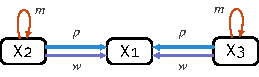
\includegraphics[width=5.5cm,keepaspectratio]{fig_flows1.pdf}
\end{center}
\caption{The data flows of program~\ref{lst:simple-dfg-1}.}\label{fig:simple-dfg-1}
\end{subfigure}\\[1em]
\begin{subfigure}{.45\textwidth}
\centering\begin{minipage}{.7\textwidth}
\begin{implisting}*[]
X1=1;
while(X2)
  X1=X1+X1
\end{implisting}
\end{minipage}
\caption{An exponential program.}\label{lst:simple-dfg-2}
\end{subfigure}\hfill
\begin{subfigure}{.45\textwidth}
\begin{center}
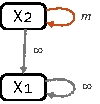
\includegraphics[width=2cm,keepaspectratio]{fig_flows2.pdf}
\end{center}
\caption{The data flows of program~\ref{lst:simple-dfg-2}.}\label{fig:simple-dfg-2}
\end{subfigure}\\[1em]
\begin{subfigure}{\textwidth}
\centering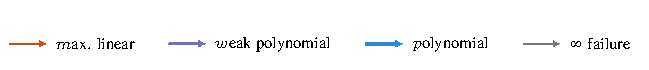
\includegraphics[width=\textwidth,keepaspectratio]{fig_flows3.pdf}
\end{subfigure}
\caption[Simple imperative programs and their corresponding data flow graphs]{
Simple imperative programs and their corresponding data flow graphs.
Edges below ∞ represent acceptable value growth.
In the left program, all variable values grow at most polynomially, \ie satisfactorily.
In the right program, variable \pr|X1| grows exponentially.
This is \enquote{too fast} for a polynomial bound.}
\label{fig:dfg-ex}
\end{figure}

\paragraph*{Analysis result and derivability.}
If all final values can be bounded by polynomial, then the input program is \emph{derivable}.
The flow calculus assigns an \emph{mwp-bound} to every variable of a derivable program.
An mwp-bound is an expression, in terms of the inputs, that characterizes the value growth of a single variable.
If a derivable program terminates, the soundness theorem of the flow calculus~\cite[p. 11]{jones2009} guarantees that the variable value growth is polynomially-bounded.
The result is sound but not complete---
not all satisfactory programs can be captured, but on success we can prove the result with a derivation.
Since the analysis omits termination, this is a partial correctness guarantee.

The flow calculus offers no guarantee to programs that are not derivable;
their variable value growth is \emph{unknown}.
A program always fails if some variable value grows \enquote{too fast}, \eg exponentially.
Failure may also arise from inability to express satisfactory behavior.
This is a built-in limitation of the flow calculus;
and more broadly, a common limitation among related systems~\cite[p. 2]{baillot2015}.
The flow calculus alleviates the issues with nondeterministic inference rules.
The nondeterminism increases expressiveness, to capture a larger class of programs.
But one program may admit multiple derivations, which in turn complicates the analysis procedure.
A program is derivable if there exists a derivation without an ∞ coefficient.

\subsubsection{Loop specifications for formal guarantees}
\label{subsec:specs}

Formally verifiable programs are defined as precise mathematical models through specifications.
Verifying the program requires giving a proof that the program satisfies its specification.
The motivation for using formal methods is the strength of guarantees it provides.
In contrast to tests and inspection, a proof conclusively ensures behavioral correctness at the modeled level of abstraction.

\paragraph*{Specifications.}
A {specification} is a formal contract with three components.
\begin{enumerate*}
    \item \emph{Precondition} \(P\), is the initial logic expressions assumed to hold before entering the loop.
    \item Program, \pr|loop b C|, performs command \pr|C| until the expression \pr|b| becomes false.
    \item \emph{Postcondition} \(Q\), is the final logic expressions asserted to hold after the loop terminates.
\end{enumerate*}
Using a {Hoare triple}~\cite{hoare1969}, we can express the specification as \(\Hoare{P}{\prm{loop b C}}{Q}\).
The implementation of the program is correct if we can construct a proof that shows the program satisfies its specification in all states.
A correctness proof requires verifying that every computation terminates, every call to another procedure satisfies its preconditions, and the postcondition holds at program termination~\cite{furia2010}.
For an example of specifications, refer to Appendix~\ref{app:sec:verified}.

\paragraph*{Relating postconditions and loop invariants.}
A postcondition is a higher-level view describing the program goal.
In case of loops, a \emph{postcondition} is a conditions that must hold after the loop terminates.
The postcondition inference problem can be expressed informally as follows.
Given a precondition \(P\) (in our formulation a constant true, \(\top\)), and a program \pr|loop b C|,
the inference problem involves finding a postcondition \(Q\) that satisfies the inference rule
\begin{prooftree} %! suppress = EscapeAmpersand
\hypo{P = \top,
    \Hoare{\prm{b}}{\prm{C}}{\top},
    \lnot\prm{b} \rightarrow Q
    & \vdash \prm{loop b C} }
\end{prooftree}.
Postconditions inferred using the flow calculus are provable by the soundness theorem.
However, pre- and postcondition alone are typically too weak to prove a program correct.
Loop invariants are often necessary to make the specification provable.

An \emph{invariant} describes an assertion about a program location that must be true for every program state reaching the location~\cite{furia2010,nguyen2022}.\footnote{A postcondition is also an invariant; for clarity, we always refer to a postcondition as such and use `invariant` to refer to an inductive loop invariant.}
A {loop invariant} is a weakened form of the postcondition~\cite{furia2010}.
An invariant is {inductive} if it holds the first time the location is reached and is preserved in every cycle returning to the location~\cite{sankaranarayanan2004}.
Verifying loops requires discovering {sufficiently strong} inductive loop invariants to prove the specification.
For an invariant to be sufficient, it must be weak enough to be derived from the precondition and strong enough to conclude the postcondition.

Inductive loop invariants and postconditions are symbiotic: the discovery of one assists finding the other~\cite{furia2010}.
Every invariant is necessarily a (weak) postcondition, as it must hold at termination, but a postcondition must not be invariant.
For example, given natural numbers \pr|i| and \pr|n|, the loop \prc|for(i=0;i<n;i++) i++;| has an invariant \(0 \leq \prm{i} \leq \prm{n}\) and a postcondition \(\prm{i}=\prm{n}\).
Invariant inference techniques may assume preconditions and postconditions are known.
However, this assumption is impractical, since manually adding specifications to code fragments is non-trivial.

\subsection{Technical Preliminaries of the Flow Calculus}
\label{sec:calc}

\begin{figure}[H]
\centering
\scalebox{.88}{\begin{tikzpicture}[align=center,
arrow/.style={thick,arrows={-Latex[width=6pt, length=4pt]}},
label/.style={midway,fill=white}]
\newcommand\lbl[2]{\textit{#1} (\autoref{#2})}
\newcommand\vtx[2]{\textbf{#1} (\autoref{#2})}

\path (0, 0) node (A) {\vtx{loop}{subsec:language}}
++(0,-2.0) node[text width=10cm] (B) {\vtx{program analysis with flow calculus}{subsec:matrices}}
++(0,-3.7) node (C) {\vtx{evaluation}{sec:enhancements}}
++(0,-3.0) node (D) {\vtx{postconditions}{sec:analysis}};

\draw[cdafny,line width=5pt,solid]($(C.north west)+(-1.5,0.4)$)  rectangle ($(D.south east)+(1.5,-0.4)$);
\draw[black,thick,densely dashed,line cap=round]($(C.north west)+(-1.5,0.4)$)  rectangle ($(D.south east)+(1.5,-0.4)$);

\draw [arrow,sbase03,arrows={{Circle[open]}-Latex[width=6pt, length=4pt]}] (A) -- (B) ;
\draw [arrow,sbase03] (B) -- node[label,yshift=7pt]  {\lbl{mwp-matrix}{subsec:mat-decode}} (C);
\draw [arrow,sbase03] (C) -- node[label] {\lbl{mwp-bounds}{subsec:interpreting-mwp-bounds}}(D);
\end{tikzpicture}}

\caption[The mwp-analysis workflow]{The mwp-analysis workflow.}
\label{fig:pc-workflow}
\end{figure}

The \autoref{fig:pc-workflow} illustrates the complete analysis workflow.
The boxed region highlights the steps and enhancements introduced in this paper.
The region outside the box refers to the existing techniques we build on.

The analysis takes as input an imperative loop (\autoref{subsec:language}).
We analyze the loop using the inference rules of the flow calculus (\autoref{subsec:matrices}).
As output, the analysis produces an \emph{mwp-matrix} (\autoref{subsec:mat-decode}).
Our enhancements involve {evaluating} these mwp-matrices.
We define first an {evaluation procedure} (\autoref{subsec:eval}) that enables extracting optimal mwp-bounds from mwp-matrices,
and in more cases than previously (\autoref{subsec:bounds-at-failure}).
This provides the postconditions that address the problem formulation of~\autoref{subsec:overview}.

\subsubsection{Imperative language of input programs}
\label{subsec:language}

\begin{definition}[Imperative language]\label{def:lang}
Letting natural number variables range over \pr|X| and \pr|Y| and boolean expressions over \pr{b},
we define \emph{expressions} \pr|e|, and \emph{commands} \pr|C| as follows
%! suppress = MissingImport
\begin{align*}
    \text{\pr|e|} \coloneqq{ }&
    \text{\pr| X|} \BNF
    \text{\pr|X - Y|} \BNF
    \text{\pr|X + Y|} \BNF
    \text{\pr|X * Y|} \\
    \text{\pr|C|} \coloneqq{ }&
    \text{\pr| skip|} \BNF
    \text{\pr|X = e|} \BNF
    \text{\pr|if b then C else C|} \BNF
    \text{\pr|while b C|} \BNF
    \text{\pr|loop X C|} \BNF
    \text{\pr|C;C|}
\end{align*}
The command \pr|loop X C| means \enquote{do \pr|{C}| \pr|X| times} and the variable \pr|X| is not allowed to occur in command \pr|C|.
Command \pr|C;C| is for sequencing.
We write \enquote{program} for a series of commands composed sequentially.
\end{definition}
We implicitly convert between conventional \prc|for| loops and \pr|loops| of the imperative language in examples.
The values of boolean expressions do not matter.
For emphasis, we substitute \pr|b| with \pr|*| in control expressions.
Although the base language is rudimentary, it captures a core fragment of conventional mainstream programming languages, like C and Java.
Our technique applies to all languages sharing the same core, including intermediate representations.
Similarly, the approach is applicable even if a programming language provides little structure.

\subsubsection{About construction of mwp-matrices}
\label{subsec:matrices}

How mwp-matrices are constructed is not crucial for the developments of this paper.
The construction procedure is well-established in literature~\cite[Sect. 5--6]{jones2009} and~\cite[Sect. 2--3]{aubert20222}.\footnote{Our work assumes the variant described in~\cite{aubert20222}.}
We give a brief overview, but make no adjustment to the construction procedure.
Rather, mwp-matrices are our inputs of interest.
We focus on \emph{interpreting} the information they encode.

During matrix construction, the flow calculus assigns matrices to commands of the input program.
The procedure resembled typing, except the \enquote{types} are complicated matrices.
An \emph{mwp-matrix} \(M\) captures data flow facts about the analyzed program \(\mathcal{C}\).
The matrices track, through flow coefficients, how data flows in variables between commands.
What coefficients are assigned is determined by the \emph{inference rules} of the flow calculus.
The relevant inference rules are included in Figures~\ref{fig:rules-expressions} and~\ref{fig:rules-loops}.\footnote{
    To ease the presentation, we show rules of the original flow calculus~\cite{jones2009}. These rules are consistent with the enhanced variant~\cite{aubert20222} we build on.}
To trade precision for efficiency, the flow calculus omits evaluating loop iteration bounds and reasoning about termination and control expressions, overestimating their effect.
At conclusion, the flow calculus assigns \underline{one} mwp-matrix to the analyzed program, \(\vdash\mathcal{C} : M\).
It contains all derivations of the input program in one (complex) data structure.

\begin{figure}[h]
    \begin{center}
        %! suppress = EscapeUnderscore
        \begin{prooftree}[small]
            \infer0[E2]{
                \vdash \prm{e} : \{_{\,i}^{w} \mid \prm{X}_i \in \var(\prm{e}) \}}
        \end{prooftree}\hfill%
        %! suppress = EscapeUnderscore
        \begin{prooftree}[small]
            \hypo{\vdash \prm{X}_i : V_1}
            \hypo{\vdash \prm{X}_j : V_2}
            \infer2[E3]{
                \vdash \prm{X}_i + \prm{X}_j : pV_1 \oplus V_2}
        \end{prooftree}%
        \hfill%
        %! suppress = EscapeUnderscore
        \begin{prooftree}[small]
            \hypo{\vdash \prm{X}_i : V_1}
            \hypo{\vdash \prm{X}_j : V_2}
            \infer2[E4]{\vdash \prm{X}_i + \prm{X}_j : V_1 \oplus pV_2}
        \end{prooftree}
    \end{center}
    \caption[A selection of flow calculus rules for assigning vectors to expressions.]
    {A selection of flow calculus rules for assigning vectors to expressions.
    A {variable} is denoted as \(\prm{X}_i\) where the \(i\) refers to an index of a matrix column
        (\resp \(\prm{X}_j\) for the \(j\)th column).
        In rules E3 and E4, a vector of coefficients is denoted by \(V_n\).
        In other words, the rules assign vectors of coefficients to variables.
        Three rules can be used to analyze a single expression.
        The nondeterminism of the flow calculus comes from these inference rules.
    }
    \label{fig:rules-expressions}
\end{figure}

Nondeterminism is necessary to improve the expressive power of the flow calculus, but complicates the analysis procedure.
There are the three rules (\autoref{fig:rules-expressions}) to analyze an expression of binary addition\footnote{
    Similar rules exist for subtraction, and multiplication is always handled by E2.}, like \pr|X1 + X2|.
Informally, the rule E2 says \enquote{we can always assign a \(w\) coefficient to all variables in the expression}.
Although such constant treatment seems  potentially harmful, the inference rules for analyzing commands (\autoref{fig:rules-loops}) ensure only acceptable data flow patterns are accepted as derivable.
The rule E3 says \enquote{the vector of the left operand is multiplied by a polynomial coefficient.}
The \(p\)-coefficient tracks the fact that certain data flow patterns might not be polynomially bounded~\cite[p. 13]{jones2009}.
Applying the rules to a vector propagates the effect to all variables that are transitively dependent on the left operand.
Rule E4 is similar to E3, except the \(p\) coefficient is applied to the right operand.
Thus, three different derivation can arise from one expression, and from every command that contains the expression.
Going forward, we omit the details of these rules and instead refer to them by a mapping \(0 \mapsto \text{E4}, 1 \mapsto \text{E3}, 2 \mapsto \text{E2}\).

\subsubsection{Our starting point of interest: interpreting mwp-matrices}
\label{subsec:mat-decode}

An mwp-matrix represents the derivations of an analyzed program.
Before diving into full mwp-matrices, this section describes its \emph{elements}.

\paragraph*{Basic terms.}
Flow coefficients---described in \autoref{subsec:flow-calc-intro}---are the core building blocks of mwp-matrices.
The flow coefficients are elements of the finite set \(\text{\textsc{mwp}}^\infty \triangleq \{0, m, w, p,\infty\}\).
A \emph{domain} \(\mathcal{D} \triangleq \{0, 1, 2 \}\) is a bidirectional map of the flow calculus inference rules.
In other words, the domain members can be translated to flow calculus inference rules (E2--E4) and vice versa.
The \emph{degree} of choice, \(k : \mathbb{N}\), is a counter of derivations.
The degree represents the number of times a derivation choice must be made during program analysis.
The degree is precisely equal to the count of binary arithmetic operations whose operator is either \(+\) or \(-\).

\begin{definition}[Derivation choice]
    Letting \( \mathcal{D} \) be a domain and \( k \in \mathbb{N} \) be the degree of choice,
    we define a derivation choice as \( \delta(i, j) \), where \( i \subseteq \mathcal{D} \) and \( j \leq k \).\end{definition}
A derivation choice, denoted by \(\delta\), represents the nondeterminism of the flow calculus.
%It is another core building block of mwp-matrices.
We call \(i\) the \emph{value} and \(j\) the \emph{index} of the derivation choice.
Informally, it captures that an inference rule \(i\) is applied at program point \(j\).
%The value indicates the selected mwp-calculus inference rule and index the program point where the rule is applied.

\begin{definition}[Derivation choice sequence]
    Letting \(k\) be the degree of choice,
    we define a derivation choice sequence as \(\Delta = (\delta_1, \delta_2, \dots, \delta_{k'})\)
    where \(0 \leq k' \leq k \). % TODO: unique + sorted
\end{definition}
Since a program is a \emph{series} of commands, correspondingly we must have \emph{sequences} of derivation choices, denoted as \(\Delta\).
Simple data flow patterns do not require making derivation choices;
therefore \(\Delta\) can be empty.
There are two restrictions on \(\Delta\).
First, an index \(j\) is allowed to occur at most once in a sequence, \ie the indices in a sequence must be unique.
Second, the sequence is sorted by the index in ascending order.
These restrictions support efficient computation during matrix construction.
Since we are only concerned with {interpreting} mwp-matrices, we assume every \(\Delta\) satisfies the uniqueness and order properties by construction.
By \autoref{fig:rules-expressions}, it is evident that one variable can be assigned multiple coefficients.
The fact that \(\Delta\) reduces to a particular coefficient is represented in a \emph{monomial}.

\begin{definition}[Monomial]\label{def:mono}
Letting \(\alpha \in \text{\textsc{mwp}}^\infty\) be a coefficient and \(\Delta\) be a sequence of derivation choices,
we define a monomial as \((\alpha, \Delta)\).
\end{definition}

\noindent
A monomial in the flow calculus is disjoint from the classic notion of monomials.
For example, both \(m.(\delta(0,0),\delta(2,1))\) and \(0\) are valid monomials by definition.
The former says \enquote{if we apply rule 0 then rule 2 (at indices 0 and 1, resp.) then we obtain an \(m\) coefficient}.
The latter says \enquote{no matter the choice, we always obtain a \(0\) coefficient}.
Finally, the fact that {different \(\Delta\)} reduce to {different coefficients} is represented by a \emph{polynomial structure}.

\begin{definition}[Polynomial structure]
    We define a polynomial structure as a sequence of monomials
    \(\big(0,(\alpha_1,\Delta_1)\), \((\alpha_2,\Delta_2)\), \(\dots\), \((\alpha_m, \Delta_m)\big)\) where \(m \geq 0\).
\end{definition}

\noindent The polynomial structure is prefixed by \(0\)-monomial to ensure it is always non-empty.
\textbf{The elements of an mwp-matrix are polynomial structures.}

\subsubsection{Decoding an mwp-matrix by example}
\label{subsec:read-mat}

An mwp-matrix \(M\) associates variables with polynomial structures.\footnote{
    For clarity and compactness, we omit needless \(0\)'s, \(\delta\)-symbols, and delimiters when displaying mwp-matrices.}
This association is defined by position.
The matrix size is determined by the number of program variables, such that for \(n\) variables, the matrix size is \(n \times n\).
The matrix is labelled by the variables. % (sometimes implicitly).
An mwp-matrix is interpreted {column-wise}.
The data-flow facts about a variable at column \(j\) are collected in the polynomial structures at rows \(i=(1, \ldots, n)\) in \(M_{ij}\).

\begin{example}[mwp-matrix of \explain]\label{ex:mat}
Consider the mwp-matrix of \explain.

\begin{center}
\begin{minipage}{\linewidth}
\begin{minipage}{.28\linewidth}
\begin{implisting}*[label={lst:pt-fail},escapeinside=||]
for(i=0;i<X1;i++)
{ X3=X2*X2;
  X3=X3+X5; |\circledc{1}|
  X4=X4+X5; |\circledc{2}| }
\end{implisting}
\end{minipage}%
\hfill : \hfill%
\scalebox{.8}{\(%! suppress = EscapeAmpersand
\begin{pNiceMatrix}[first-row,first-col]
& \prm{X1} & \prm{X2} & \prm{X3} & \prm{X4} & \prm{X5} \\
\prm{X1} & m & 0 & p(0,0),p(1,0)         & p(0,1),\infty(1,1),\infty(2,1)  & 0 \\
\prm{X2} & 0 & m & w(0,0),p(1,0),w(2,0)  & \infty(1,1),\infty(2,1)         & 0 \\
\prm{X3} & 0 & 0 & m                     & \infty(1,1),\infty(2,1)         & 0 \\
\prm{X4} & 0 & 0 & 0                     & m,\infty(1,1),\infty(2,1)       & 0 \\
\prm{X5} & 0 & 0 & p(0,0),m(1,0),w(2,0)  & p(0,1),\infty(1,1),\infty(2,1)  & m \\
\end{pNiceMatrix}\)}
\end{minipage}
\end{center}

We mark the program points where a derivation choice must be made as \circledc{1} and \circledc{2}.
The program points correspond to indices 0 and 1, respectively.
These points give the mwp-matrix a degree of 2.
The addition expressions are analyzed by the inference rules of~\autoref{fig:rules-expressions}.
The mwp-matrix contains derivations choices at columns \pr|X3| and \pr|X4| because they are the data-flow targets of the additions.
Correspondingly, in~\autoref{fig:ll-dfg}, the variables are targets of dependence edges.

\begin{figure}[H]
\centering
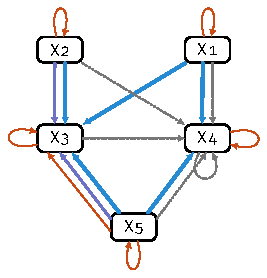
\includegraphics[width=6cm,keepaspectratio]{fig_lucid.pdf}
\caption[A data-flow graph of \exname]{A data-flow graph of \exname.}
\label{fig:ll-dfg}
\end{figure}

\noindent{}Variables \pr|X1|, \pr|X2|, and \pr|X5| are assigned at most \(m\){ }coefficients.
An \(m\)-flow at the mwp-matrix diagonal means the variable depends on its (own) initial value.
Since the program has no commands that would introduce multiple derivations on these variables, their polynomial structures are simple coefficients.
%Exactly one mwp-bound describes each of the three variables.
Variable \pr|X3| shows varying dependencies on \pr|X1|, \pr|X2|, and \pr|X5| at corresponding rows.
The coefficients indicate that the dependencies are at most polynomial (similarly observable in the \textsc{dfg}).
The absence of ∞ means the value growth of \pr|X3| is acceptable in all derivations.
Variable \pr|X4| is assigned ∞ in some derivations.
Intuitively, this is because the value of \pr|X4| accumulates at each loop iteration and its value growth is potentially problematic.
The ∞-flow signals that some derivations fail and flags \pr|X4| as the source of failure.
However, this is the current extent of our capabilities to describe \pr|X4|~\cite{aubert2023b}.
\end{example}

\noindent This paper develops enhanced strategies to extract more precise information from mwp-matrices.
$\poly_2$Although we show only compact cases, an mwp-matrix captures \(3^k\) derivation choices where \(k\) is the degree.
Clever solutions are necessary to explore and interpret the mwp-matrix data efficiently, but have been missed by previous flow calculus refinements~\cite{aubert20222,aubert2023b}.

\subsubsection{Interpreting mwp-bounds}
\label{subsec:interpreting-mwp-bounds}

The mwp-matrix columns encode the variable value growth bounds.
An mwp-bound is an expression of form $\max(\vec{x}, \poly_1(\vec{y})) + \poly_2(\vec{z})$.
Variables characterized by $m$-flow are listed in $\vec{x}$; $w$-flows in $\vec{y}$, and $p$-flows in $\vec{z}$.
Variables characterized by $0$-flow do not occur in the expression.
No bound exists if some variable is characterized by ∞.
The $\poly_1$ and  are \emph{honest polynomials}, build up from constants and variables by applying $+$ and $\times$. % (\cf~\autoref{app:sec:hp} for details).
The variables with \(w\)-flow occur in $\poly_1$ and variables with \(p\)-flow in $\poly_2$.
Any of the three variable lists might be empty, and $\poly_1$ and $\poly_2$ may not be present.
When characterizing value growth, an mwp-bound is approximative.
It excludes precise constants and degrees of polynomials.
The mwp-bound is a monotonic over-approximation, \ie it does not decrease if variable value decrease over subtraction.
A program \emph{bound} is a conjunction of its variables' mwp-bounds.
\autoref{ex-bounds} shows illustrative cases of mwp-bounds.
The differences between the bound forms are discussed in Sections~\ref{subsec:categories} and~\ref{subsec:disclaimer}.

\begin{note}
    For variable \pr|X| and an mwp-bound \(W\), we write \(\prm{X'} \leq W\) to denote the mwp-bound of variable \pr|X|.
    We use the overloaded notation \pr|X'| to refer to the variable's final value.
    Variables in \(W\) always refer to initial values.
\end{note}

\begin{example}\label{ex-bounds}
The mwp-bound (on left) is interpreted as, {the \emph{final value} of\ldots}

\noindent\hfill\begin{tabular}{@{}rl@{\hskip 0.1in}l@{}}
\(\prm{X2'} \leq \prm{X2} \) & & {\ldots \prc|X2| is bounded linearly by its initial value.} \\
\(\prm{X3'} \leq \max(\prm{X3},\prm{X2}+\prm{X5})\) & & {\ldots \prc|X3| is bounded by a weak polynomial in \prc|X3| or \(\prm{X2}+\prm{X5}\).} \\
\(\prm{X4'} \leq \max(\prm{X4})+\prm{X1}\times\prm{X5}\) & & {\ldots \prc|X4| is bounded by a polynomial in \prc|X4| and \(\prm{X1}\times\prm{X5}\).}
\end{tabular}
\end{example}

\subsection{Variable-Guided Matrix Exploration}
\label{sec:enhancements}

\subsubsection{Addressed limitations}
\label{subsec:enhancements}

We introduce two solutions to address current limitations of the flow calculus. % of mwp-bounds.

\begin{enumerate}
    \item An mwp-matrix \emph{evaluation strategy}, to efficiently determine if an individual variable admits an mwp-bound of specific form.
    \item Improved \emph{derivation failure handling}, to identify variables that maintain acceptable value growth in presence of whole-program derivation failure.
\end{enumerate}

\noindent The nondeterminism of the flow calculus permits capturing more programs, but creates a potential state explosion problem.
Effectively handling this aspect becomes critical in the second analysis phase, where an mwp-matrix is \emph{evaluated} to find mwp-bounds of variables.
The first challenge is finding the derivation choices that do not produce failure.
The second challenge is determining the coefficients assigned to each variable.
The coefficients are not obvious from the derivation choices of an mwp-matrix;
rather, they require an application.
An \emph{application} reduces the polynomial structures to simple coefficients, which then leads to derivation failure or yields a program bound.

A brute force solution iterates all derivations and applies all choices to observe the result.
However, such naive solution is impractical, due to latency and a potential yield of exponentially many program bounds.
The ideal solution should find the optimal bound (if one exists) and without the redundancy of iterating every derivation.

The evaluation strategy we present operates as follows.
It takes the \emph{unwanted} derivation choices then negates them.
The evaluation result the captures the \emph{permissible} choices.
The term permissible is abstract -- the meaning depends on what is unwanted.
For example, if the derivation choices of ∞ coefficients are unwanted,
the permissible choices are those that avoid failure, \ie non-∞.
The result of an evaluation is a \emph{disjunction of choice vectors} that compactly capture the permissible derivation choices.

\begin{definition}[Choice vector]
    Letting \( \mathcal{D} \) be a domain and \( k \in \mathbb{N} \) be a choice degree,
    we define a choice vector as \( \vec{C} = (c_1, c_2, \ldots, c_k) \),
    where \( c_i \subseteq \mathcal{D} \) and \( c_i \neq \emptyset \) for all \( i \in \{1, 2, \ldots, k\} \).
\end{definition}
We show choice vectors in Examples~\ref{ex:derivable},~\ref{ex:wbound}, and~\ref{ex:whl}.

\subsubsection{Evaluation for identifying derivable programs}
\label{subsec:eval}

The precise mwp-matrix evaluation strategy is presented in~\autoref{alg:algo} and we describe it here informally.
The evaluation is parametric on three inputs:
\begin{enumerate*}[label=(\roman*)]
\item the degree of choice \(k\),
\item domain \(\mathcal{D}\), and
\item a set of unwanted derivation choice-sequences, \(\mathcal{S} = \{\Delta_1,\ldots,\Delta_n\}\) where \(n \geq 0\).
\end{enumerate*}
Observe that all parameters are obtained from an mwp-matrix, but the mwp-matrix or its coefficients are \underline{not} used.
The evaluation returns a list of choice vectors.
In the maximally permissive case, the result is a single choice vector permitting everything.
If no result exists or no choice is necessary, the result is an empty list.
These outcomes are handled as base cases (Lines~\ref{alg:step0}--\ref{alg:step0end}).
All interesting evaluations fall between these extremes.

\begin{algorithm}
    \caption{mwp-matrix evaluation}
    \label{alg:algo}
    \textbf{Input}:
    degree \(k\) (\(\mathbb{N}\)),
    domain \(\mathcal{D}\) (set),
    derivation choice-sequences \(\mathcal{S}\) (set)\\
    \textbf{Output}: choice vectors \(\mathcal{C}\) (list)
    \begin{algorithmic}[1]
        \State \(\mathcal{C} \gets \varepsilon \)
        \LineComment{Handle base cases}
        \If {\(k = 0\) \textbf{or} \(|\mathcal{D}|\leq 1\) \textbf{or} \(\mathcal{S} = \emptyset\)}\label{alg:step0}
        \If {\(\mathcal{S} = \emptyset\)}
            \State Create \(\vec{c} \coloneqq\) ChoiceVector(\(k, \mathcal{D}\))
            \Comment{\(k\)-length vector of elements in \(\mathcal{D}\)}
            \State \(\mathcal{C} \gets \vec{c} \dblcolon\mathcal{C} \)
        \EndIf
        \State \Return \(\mathcal{C}\)\label{alg:step0end}
        \EndIf
        \LineComment{Step 1: Simplify \(\mathcal{S}\) until convergences}
        \Do \; Capture initial \(\text{\textit{size}} \coloneqq |\mathcal{S}|\)
        \Comment{\(\mathcal{O}(\mathcal{S}^3)\)}
        \State \(\mathcal{S} \gets \textsc{Simplify}(\mathcal{S})\)\label{alg:step1}
        \doWhile{\text{\textit{size}} \(\neq |\mathcal{S}|\)}
        \LineComment{Step 2: Generate choice vectors}
        \State Compute \(P \coloneqq\) the product of sequences in \(\mathcal{S}\)\label{alg:step2}
        \ForAll{paths \(p\) in P} \Comment{\(\mathcal{O}(\prod_{s \in \mathcal{S}} |s|)\)}
        \State Create \(\vec{c} \coloneqq\) ChoiceVector(\(k, \mathcal{D}\))
        \ForAll{\((i, j)\) in \(p\)}  \Comment{\(\mathcal{O}(|\mathcal{S}|)\)}
        \State Remove \(i\) at \(\vec{c}_j\)
        \EndFor
        \If {\(\forall j, \vec{c}_j \neq \emptyset \)}
            \State \(\mathcal{C} \gets \vec{c} \dblcolon\mathcal{C} \)\label{alg:add}\label{alg:step2end}
        \EndIf
        \EndFor
        \State \Return \(\mathcal{C}\)
    \end{algorithmic}
\end{algorithm}

The evaluation operates in two steps.
First it simplifies \(\mathcal{S}\) to the minimal length, non-empty sequences while preserving its effect.
Then, it generates the choice vectors by negating the remaining unwanted choices.
The procedure is practically efficient because simplification eliminates redundancy before the choice vector are generated.
Internally, it benefits from the finiteness of the domain and from having advance complete knowledge of all derivation choices.

The simplification step (Line~\ref{alg:step1}) is crucial.
It must be sound and complete to ensure all distinct derivation patterns are preserved in \(\mathcal{S}\),
but also reduces \(\mathcal{S}\) to a minimal set. % to make the subsequent step efficient.
Different simplifications are applied on \(\mathcal{S}\) iteratively until convergence, including the following.

\begin{description}

    \item[Remove super-sequences.] When a sequence leads to an unwanted outcome, every longer sequence producing the same outcome is redundant.
    For example, if \(\mathcal{S}\) contains \(((0,0),(0,1),(1,2))\) and \(((0,1))\) we remove the longer sequence.

    \item[Head-elimination.] If many non-singleton sequences differ only on their head element value, and the values cover the domain \(\mathcal{D}\), then the head is redundant.
    The sequences can be replaced by one sequence without the head element.
    For example, the sequences \(((0,0)(1,1))\), \(((1,0)(1,1))\), \(((2,0)(1,1))\) can be replaced by \(((1,1))\).

    \item[Tail-elimination.] By symmetry, the same as above, but on the tail element.

\end{description}

The generation step (Lines~\ref{alg:step2}--\ref{alg:step2end}) produces the choice vectors.
They are constructed by computing the cross product of \(\mathcal{S}\).
We take one derivation choice from each sequence, then eliminating those choices.
This prevents choosing any unwanted sequence completely.
If the choice vector elements are non-empty after elimination, we appended the choice vector to the result (Line~\ref{alg:add}).
We have annotated the computational costs of the iterative steps in~\autoref{alg:algo}.
The algorithm obviously terminates.
Since the generation step involves a product, it is a source of potential inefficiency.
However, we have not encountered natural programs where the simplification does not reduce \(\mathcal{S}\) sufficiently to make the generation step problematic.
A full implementation of the algorithm is included in our artifact, and described in the \href{https://statycc.github.io/pymwp/choice}{documentation} of pymwp.\footnote{See: \url{https://statycc.github.io/pymwp/choice}}

\begin{example}[\exname is derivable]\label{ex:derivable}
In \autoref{ex:mat}, the distinct monomials that cause failure are \(\infty.\delta(1,1)\) and  \(\infty.\delta(2,1)\).
The mwp-matrix degree is \(k=2\), the domain is \(\mathcal{D}=\{0,1,2\}\), and the unwanted derivation choice-sequences are \(\mathcal{S} = \{ ((1,1)), ((2,1)) \}\).
The evaluation returns a choice vector \(\big(\{0,1,2\}, \{0\}\big)\) witnessing successful derivation choices.
The choice vector communicates that we can select any derivation rule to analyze command \circledc{1}, but must apply \enquote{inference rule 0} (E4) at command \circledc{2}.
\end{example}

The application of a choice vector requires making a selection at each vector index, then applying the selections to the polynomial structures of the mwp-matrix.
A monomial evaluates to \(\delta(i, j) = \alpha\) if the \(j\)th choice is \(i\), and \(0\) otherwise.
A polynomial structure evaluates to its maximal coefficient.
Thus, the application produces the maximal coefficient among the monomials (\cf~\autoref{ex:whl}).

\subsubsection{Variable projection and querying mwp-bounds}
\label{subsec:query}

Until now, the flow calculus of mwp-bounds has been restricted to deriving mwp-bounds for all variables concurrently.
For postcondition inference, we want to obtain information about \emph{individual} variables.
Since~\autoref{alg:algo} does not require mwp-matrices or coefficients as input, it can be directly reused for variable-specific evaluations.

Analyzing variable \(\prm{X}_j\) requires taking derivation choices only from column \(j\), instead of the entire mwp-matrix.
To determine if a variable admits a particular form of mwp-bound, we issue \enquote{queries} against the evaluation procedure,
altering the derivation choices provided as parameter \(\mathcal{S}\).
For example, to find derivations with at most \(m\) coefficients (and whether they exist), we take the derivation choices from monomials whose coefficient are in \(\{w, p,\infty\}\).
If the evaluation returns a choice vector, it specifies the derivations where the variable is assigned an mwp-bound of at most \(m\) coefficients.
Bounds with at most \(w\) or \(p\) can be queried similarly, by adjusting \(\mathcal{S}\).

\begin{example}[Variable \texttt{X3} is bounded by at most $w$ coefficients]\label{ex:wbound}
In \autoref{ex:mat}, variable \pr|X3| does not have a derivation with at most \(m\) coefficients.
This can be determined by evaluation of the distinct choices in column \pr|X3| with \(\{w, p, \infty\}\) coefficients,
\ie \(\mathcal{S} = \{ ((0,0)),((1,0)),((2,0)) \}\).
This evaluation does not return a choice vector.
However, an mwp-bound of at most \(w\) exists, by the choice vector \(\big(\{2\}, \{0,1,2\}\big)\).
\end{example}

\noindent Variable query is safe for derivable programs, because all variables are guaranteed to have an mwp-bound by the soundness theorem of the flow calculus~\cite[p. 11]{jones2009}.
Additional caution is needed when a program is not derivable.

\subsubsection{Variable mwp-bounds in presence of failure}
\label{subsec:bounds-at-failure}

Derivation failure arises from the inference rules of commands \pr|while| and \pr|loop|, in~\autoref{fig:rules-loops}.

\begin{figure}[h]
\begin{center}
\begin{prooftree}[small]
\hypo{\vdash \text{\pr|C|} : M}
\infer[left label={\(\forall i, M_{ii}^* = m\)}]1[L]{
\vdash \prm{loop X}_\ell\,\prm{\{C\}} : M^* \oplus \{_\ell^{p}\rightarrow j \mid \exists i, M_{ij}^* = p\}}
\end{prooftree}
\\[1.2em]
\begin{prooftree}[small]
\hypo{\vdash \text{\pr|C|} : M}
\infer[left label={\(\forall i, M_{ii}^* = m\) and \(\forall i, j, M^*_{ij} \neq p\)}]1[W]{\vdash \text{\pr|while b do  \{C\}|} : M^*}
\end{prooftree}
\end{center}
\caption{The flow calculus inference rules for commands \pr|while| and \pr|loop|.}
\label{fig:rules-loops}
\end{figure}

The interesting parts about these rules are the side conditions.
For the \pr|loop| rule (L), the side-condition says a loop can be analyzed if the coefficients at the mwp-matrix diagonal are at most \(m\).
The \pr|while| (W) rule is more restrictive.
In addition to diagonal \(m\), no \(p\) coefficients are allowed to occur anywhere in the mwp-matrix.
These side-conditions ensure variable values grow at most polynomially over repeated executions of the command body.

A program that does not satisfy the side-conditions is not derivable.
Then, variable value growth is inconclusive and no bound is assigned to its variables.
The flow calculus offers no guarantees to programs that are not derivable.
A single rogue variable can cause a whole-program derivation failure.
This treatment of failure limits the utility of the analysis.
Since our goal is to infer postconditions of loops, this restriction excludes many programs we want to analyze.

\paragraph*{Improving the failure handling.}
Our intuition is that the mwp-matrices accumulate information that permits reasoning about {certain variables} in presence of failure.
The main new idea is to \emph{isolate the failing variables} from those with acceptable behavior.
If such isolation is possible, then the remaining variables can be analyzed.
The idea is conservative because it does not change the rules of the flow calculus.
Rather, the improvement is based on leveraging fully the information already collected in mwp-matrices.
We make only the analytical adjustment illustrated in~\autoref{fig:part-prog}.
Our treatment of failure is sound by the guarantees of the original flow calculus -- explained shortly after the motivating example.

\begin{figure}
\centering
\begin{subfigure}[t]{.25\textwidth}
\begin{minipage}{\textwidth}
\begin{implisting}*[label=fail-p]
while(*) {
{ X3=X2*X2;
  X3=X3+X5;
  X4=X4+X5; }
\end{implisting}
\end{minipage}
\caption{Input program}\label{lst:whole-p}
\end{subfigure}%
\begin{subfigure}[t]{.75\textwidth}
\hfill{}:{}\hfill\scalebox{.8}{
\(\begin{pNiceMatrix}[first-row,first-col]
\CodeBefore
\cellcolor{lgrey}{3-,-3}
\Body
& \prm{X2} & \prm{X3} & \prm{X4} & \prm{X5} \\
\prm{X2} & m & \infty(0,0),\infty(1,0),w(2,0)                  & \infty(0,1),\infty (1,1),\infty (2,1) & 0 \\
\prm{X3} & 0 & m,\infty(0,0),\infty(1,0)                       & \infty(0,1),\infty (1,1),\infty (2,1) & 0 \\
\prm{X4} & 0 & \infty(1,0)                                     & \infty(0,1),\infty (1,1),\infty (2,1) & 0 \\
\prm{X5} & 0 & \infty(0,0),m(1,0),\infty(1,0),w(2,0)           & \infty(0,1),\infty (1,1),\infty (2,1) & m \\
\end{pNiceMatrix}\)}
\caption{mwp-matrix with failure}\label{fig:fail-matrix}
\end{subfigure} \\[1em]
\begin{subfigure}{.45\textwidth}
\centering
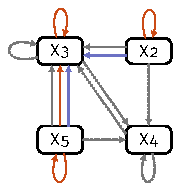
\includegraphics[width=4.5cm,keepaspectratio]{fig_dfg.pdf}
\caption{\textsc{dfg} of the mwp-matrix}\label{fig:fail-dfg}
\end{subfigure}\hfill%
\begin{subfigure}{.45\textwidth}
\centering
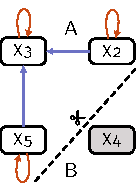
\includegraphics[width=3.2cm,keepaspectratio]{fig_cut.pdf}
\caption{Grouping and independence}\label{fig:group-part}
\end{subfigure} \\[1em]
\begin{subfigure}{\textwidth}{
\centering
\begin{minipage}{.35\textwidth}
\begin{implisting}*[label={lst:p1}]
while(*) {
  X3=X2*X2;
  X3=X3+X5; }
\end{implisting}
\end{minipage}%
\hspace{2em}%
\begin{minipage}{.35\textwidth}
\begin{implisting}*[label={lst:p2}]
while(*) {
  X4=X4+X5;
}
\end{implisting}
\end{minipage}
\caption{Sub-programs}\label{lst:sub-progs}
}\end{subfigure}
\caption[A demonstration of improved derivation failure handling]{
A demonstration of improved derivation failure handling.
The program (\ref{lst:whole-p}) is a modified version of \exname.
The variable \pr|X4| causes failure in every derivation (\ref{fig:fail-matrix}).
Starting with \ref{fig:fail-dfg}, we restrict the graph to derivations where non-failing variables can be bounded.
This reduces the edges to those shown in \ref{fig:group-part}.
The sub-program that corresponds to variables in set \(\mathsf{A}\) (\ref{lst:sub-progs}, above) is derivable.
}\label{fig:part-prog}
\end{figure}

\begin{example}[Evaluating an always failing derivation]\label{ex:whl}
The program in~\autoref{lst:whole-p} is not derivable because variable \pr|X4| fails in every derivation.
The area of failure, that we want to isolate, is shaded in the mwp-matrix of~\autoref{fig:fail-matrix}.
Not all variables are problematic.
There is no dependency from \pr|X4| to variables \pr|X2| and \pr|X5| (row \pr|X4|).
Variable \pr|X3| is more complicated due to the ∞ coefficients in column \pr|X3|.
Since we want derivations where \pr|X3| is derivable, we compute its choice vector: \(\big(\{2\}, \{0,1,2\}\big)\).
At index 0, variable \pr|X3| permits one derivation choice: 2.
Applying \((2,0)\) to the mwp-matrix, at column \pr|X3|, yields coefficients:
\(\text{\pr|X2|} \mapsto w\),
\(\text{\pr|X3|} \mapsto m\),
\(\text{\pr|X4|} \mapsto 0\), and
\(\text{\pr|X5|} \mapsto w\).
The \(0\) reveals that in every derivable case variable \pr|X3| is independent of \pr|X4|.
Therefore, variables \pr|X3|, \pr|X2| and \pr|X5| can be assigned mwp-bounds.
\end{example}

\subparagraph*{Variable grouping} (\autoref{fig:group-part}).
The whole-program derivability is first determined by~\autoref{subsec:eval}.
In the negative case, at least one variable must be failing.
Crucially, a failing variable fails in {every derivation}.
Therefore, it suffices to evaluate variables individually for at most \(p\) coefficients, by~\autoref{alg:algo}.
We group variables into two sets.
Set \(\mathsf{A}\) with variables that satisfy polynomial value growth, and set \(\mathsf{B}\) with variables that fail.
Which set each variable belongs to is determined by the existence of a choice vector.

\subparagraph*{Establishing independence from failure} (\autoref{fig:group-part}).
Recall, the \(0\) coefficients track {absence} of data flows between variables.
Thus, we can determine if sets \(\mathsf{A}\) and \(\mathsf{B}\) are data-flow independent from the \(0\)s.
We must ensure that there is no data flow \emph{from} the failure set \(\mathsf{B}\) to set \(\mathsf{A}\) in the cases where variables in \(\mathsf{A}\) are derivable.
The condition can be determined by direct inspection of the mwp-matrix.
The independence condition corresponds to a cut of the data flow graph.

\subparagraph*{Partitioning to sub-programs} (\autoref{lst:sub-progs}).
When failure independence is affirmative, we {partition} the whole-program into two sub-programs.\footnote{
    This is a conceptual step; no concrete program transformation is necessary.}
These sub-programs correspond to the data flows in sets \(\mathsf{A}\) and \(\mathsf{B}\).
No bound can be derived for the failing variables in set \(\mathsf{B}\).
Variables in set \(\mathsf{A}\) are analyzed by the standard rules of the flow calculus, which ensures soundness.
\emph{Derivability of this sub-program is the source of increase in the flow calculus expressivity.}

\subsection{mwp-bounds as Postconditions}
\label{sec:analysis}

\subsubsection{Optimal mwp-bounds by form}
\label{subsec:categories}

The enhanced flow calculus now provides a technique for postcondition inference.
We aim to compute the optimal postconditions for each variable, if they exist.
There are two unresolved concerns.
First, mwp-bounds cannot be totally ordered since some forms are incomparable.
Second, mwp-bounds of different form can evaluate to the same numeric polynomial.
For example, the three mwp-bounds
\(W_1 \equiv \max(0,\prm{X1}+\prm{X2})+0\) and
\(W_2 \equiv \max(\prm{X1},0)+\prm{X2}\) and
\(W_3 \equiv \max(\prm{X2},0)+\prm{X1}\) are all numerically equal to \(\prm{X1}+\prm{X2}\).
Therefore, reasoning about optimality requires an alternative approach.

To establish an ordering, we leverage two built-in features of the flow calculus.
The individual coefficient are ordered \(0 < m < w < p < \infty\).
Moreover, the mwp-bounds carry semantic meaning \emph{by form}.
The growth of a variable value is at most {linear} (\resp iteration-independent, iteration-dependent)
if its mwp-bound contains at most \(m\) (\resp \(w\), \(p\)) coefficients.
This gives sufficient justification for our definition of optimality.

\begin{definition}[Optimality]
    We define an order on mwp-bounds by form, by the \emph{maximal} coefficient it contains:
    \(0 < m\text{-bound} < w\text{-bound} < p\text{-bound} < \infty \text{(none)}\).
    A variable's mwp-bound is optimal if it is the least bound in this order.
\end{definition}

\noindent For example, among \( W_1, W_2\), and \(W_3\),
the \(w\)-bound \(\max(0,\prm{X1}+\prm{X2})+0\) is optimal because it contains no \(p\) coefficients.
It supplies the evidence that the variable's value growth is eventually loop iteration independent (discussed in~\autoref{subsec:disclaimer}).
The other candidates \( W_2\) and \(W_3\) are too weak to reach the same conclusion.
Finding a single derivation that admits the optimal form is sufficient.

\subsubsection{Variable postcondition search}
\label{subsec:pc-search}

When a program is derivable, or a variable is disjoint from failure,
the general procedure for deriving a variable's optimal postcondition is as follows.

\begin{enumerate}
    \item Run the mwp-matrix evaluation (\autoref{alg:algo}) iteratively.
    Construct the set \(\mathcal{S}\) from monomials whose coefficient is greater than \(m\) (next \(w\), then \(p\)).
    \item Stop at the first choice vector.
    This solution is optimal.
\end{enumerate}

\noindent
Since the search focuses on individual variables, we may want to ask whether multiple postconditions can occur concurrently.
To determine the answer, we take the intersection of their choice vectors (\autoref{def:intersect}).
A non-empty intersection specifies the derivations in which both postconditions hold.
Related questions about postconditions can be formulated similarly, as operations on choice vectors.

\begin{definition}[Choice vector intersection]\label{def:intersect}
Letting \(\vec{C_a} = (a_1, a_2,\dots,a_k) \) and \(\vec{C_b} = (b_1\), \(b_2\), \(\dots\), \(b_k)\) be choice vectors of length \(k\),
we define the intersection of \(\vec{C_a} \text{ and } \vec{C_b} \) as
\[ \vec{C_a} \cap \vec{C_b} = \begin{cases}
(a_1 \cap b_1, a_2 \cap b_2, \dots, a_k \cap b_k), & \text{ if } \not\exists i \text{ such that } a_i \cap b_i = \emptyset, \\
\emptyset, & \text{ otherwise.}\end{cases}
\]%\qedhere
\end{definition}

\begin{example}[Successful and optimal postcondition of \texttt{X3}]\label{ex:opt-derivation}
By \autoref{ex:derivable}, \exname is derivable by choice vector \(\big(\{0, 1, 2\}, \{0\}\big)\).
By \autoref{ex:wbound}, variable \pr|X3| is assigned its optimal postcondition in derivations \(\big(\{2\}, \{0,1,2\}\big)\).
The whole-program is derivable \emph{and} variable \pr|X3| is assigned its optimal postcondition in derivations defined by choices
\( \big(\{0, 1, 2\}, \{0\}\big) \cap \big(\{2\}, \{0,1,2\}\big) = \big( \{2\}, \{0\}\big) \).
\end{example}

\subsubsection{Program analysis for postcondition inference}
\label{subsec:inference}

Postcondition inference requires adjusting the imperative language (\autoref{subsec:language}) to a language of loops.
A \emph{loop program} starts with a looping command (\pr|while| or \pr|loop|) whose body is any command in the imperative language.
Using the mwp-matrix evaluation procedure, we compute postconditions for all variables that have expressible mwp-bounds.
To avoid repeated analysis, we proceed from loop nests to parent and compose mwp-matrices in a bottom-up manner. % and omit repeated analysis.
Postcondition inference of loop \(P\) is defined as follows.

\begin{enumerate}
    \item Extract all (possibly nested) loops from the program \(P\).
    \item (bottom-up) For each loop \(l\):
    \begin{enumerate}[label=(\roman*)]
    \item Run the mwp analysis to derive the mwp-matrix, \(l : M\).
    \item Using \autoref{alg:algo}, evaluate \(M\) to determine if \(l\) is derivable.
    %! suppress = MissingImport
    \begin{itemize}
        \item[] \(\triangleright\) If yes: mark every variable as satisfactory.
        \item[] \(\triangleright\) If no: mark the non-failing variables as satisfactory (\autoref{subsec:bounds-at-failure}).
    \end{itemize}
    \item Evaluate satisfactory variables for optimal postconditions (\autoref{subsec:pc-search}).
    \item Record the postconditions of satisfactory variables.
    \end{enumerate}
    \item Return the analysis result for \(P\).
\end{enumerate}

\subsubsection{Postcondition categories as descriptors of variable value behavior}
\label{subsec:disclaimer}

A language of loops restricts the kind of computations we may encounter.
The inferred postconditions can be described by the following categories.

\begin{description}

    \item[Linear.]
    A variable's mwp-bound is linear if its value does not change or it is a target of direct assignment (without arithmetic).
    Inside loops, other operations are \enquote{too strong} to retain linear behavior.
    In \exname, variables \pr|X1|, \pr|X2| and \pr|X5| are linear because their values never change.

    \item[Iteration-independent.]
    A variable is iteration-independent if its final value depends on a fixed number of iterations (\eg the first or last one) or eventually reaches a fixed point.
    Iteration independence means that, beyond the fixed point, the variable is unaffected by an increase in loop iteration count.
    Thus, iteration-independence is a quasi-invariance property.
    In \exname, if the loop iterates at least once, the final value of \pr|X3| is determined by \pr|X2| and \pr|X5|.
%This makes variable \pr|X3| iteration-independent.
%   Increasing the iteration count has no impact.
% The flow calculus distinguished this fact with the \(w\) coefficient.

    \item[Iteration-dependent.]
    Arithmetic computations involving multiple changing variables lead to iteration-dependent value growth.
    It may occur in bounded loops, but not otherwise.
    This is because a continuously increasing value may be boundable under finite iteration, but cannot be bound soundly if the loop is unbounded.
    In \explain, changing the number of times the loop iterates changes the final value of \pr|X4| respectively.
    This makes \pr|X4| iteration-dependent.

    \item[Inconclusive.]
    If no expressible postcondition exists, the variable is inconclusive.
    It characterizes cases where a variable's value growth is outside the previous three categories.
%A variable's value growth is either beyond a polynomial or inexpressible as mwp-bounds.
    In~\autoref{ex:whl}, since the loop does not terminate, the value of \pr|X4| grows in perpetuity, which marks the variable inconclusive.

\end{description}

\paragraph*{A note on numerical minimality.}
One variable may be assigned multiple incomparable mwp-bounds.
The definition of optimality does not guarantee the selected postposition is the numerical minimum by evaluation.
For example, variable \pr|X3| in \exname is assigned three mwp-bounds
\(W_1 \equiv \max(\prm{X3},\prm{X2})+\prm{X1} \times \prm{X5} \) and
\(W_2 \equiv \max(\prm{X3},\prm{X2}+\prm{X5}) \) and
\(W_3 \equiv \max(\prm{X3},\prm{X5})+\prm{X1} \times \prm{X2} \).
For purpose of this example, assume \(\prm{X1}>0\) to consider the iterative case and ignore \(W_2\).
This leaves two alternatives.
These can evaluate to distinct numeric values, yet both are equally optimal by definition.

\subsubsection{Implementing postcondition inference with \impl}
\label{subsec:implementation}

We implemented the analysis of~\autoref{subsec:inference} as an extension of the static analyzer pymwp.
    {pymwp}~\cite{aubert2023b} is an open source implementation of the flow calculus of mwp-bounds on a subset of \pr|C|.
pymwp takes as input a \pr|C| file and analyzes variable value growth in each of its functions.
Our implementation adds to pymwp a new loop analysis mode, \impl.
The loop analysis is complementary to the default function analysis mode, which we name \impf for distinction.
The primary differences are that \impl looks for {optimal} bounds by variable in a {loop},
and \impf finds existence of {any} bound for all variables in a {function}.
Though applicable to both, the paper enhancements are implemented only in \impl to enable evaluation.

During program analysis, the input file is mapped to the imperative language of~\autoref{def:lang}.
Only loops that are fully expressible in the imperative language are analyzed.
Analyzing program fragments is possible due to compositionality of the flow calculus.
Stated differently, we can apply the analysis early, even if some program parts are missing.
pymwp supports all loop constructs of \pr|C|.
The flow calculus treats the iteration space conservatively as an over-approximation.
Keywords \pr|break| and \pr|continue| have no observable impact.
Similarly, verification macros like \pr|assert| may be present, but do not impact the analysis.

When a \pr|C| loop construct is obviously bounded\footnote{For example, in \pr|for(int i=0;i<N;i++)| the iterator \pr|i| must not occur in the body and the body operations are arithmetic. Without nesting, it is clearly a finite loop.}, it is treated as a bounded loop in the flow calculus.
Otherwise, the construct is treated as an unbounded loop.
Detection of loop boundedness impacts the number of derivable variables, since a bounded loop permits iteration-dependency.
The current detection is based on loop form and it is still rudimentary.
In the future, improving the analyzer's handling of richer loop forms would yield more bounded variables.

To use the analysis results as concrete verification assertions, two more steps are required.
First, we must record the initial variable values because they are needed to express postconditions.
Next, we must complete the parts that are left implicit in mwp-bounds, like constants.
\autoref{app:sec:verified} demonstrates how we perform both steps.
In general, the postpositions provide bounding expressions \wrt input variables, with some possible omissions.
However, filling in the expression is conceptually easier than starting with no expression at all.

\subsection{Comparing Related Techniques}\label{sec:related-works}

\subsubsection{Automatic inference of specification conditions}
\label{subsec:automatic-inference}

Our work relates primarily to approaches that aim to unify software verification and complexity.
Whereas loop invariants are used in~\cite{nguyen2017} to obtain complexity results, we synthesize specification conditions starting from complexity analysis.
The bidirectionality suggests that further investigations, connecting the two topics, is warranted.
Narrowing down to specifications, automatic specification inference in general is a challenging problem~\cite{dillig2013,yu2023}.
It is common to break down the problem into smaller parts: preconditions, postconditions, and (inductive) invariants.
Inference of postconditions is the most relevant \wrt our analysis.
Although invariants inference is studied extensively in literature~\cite{karr1976,cousot1978,colon2003,sankaranarayanan2004,dillig2013,si2018,ryan2020,yao2020,yu2023,nguyen2014,nguyen2017},
existing works that intentionally target postconditions are rare~\cite{popeea2006,molina2021}.

There are a few instances that infer postconditions statically.
In~\cite{popeea2006}, show how abstract interpretation can be used to obtain a static technique for postposition analysis.
Conceptually it is close to our goals, but abstract interpretation differs considerably from the flow calculus.
Moreover, no implementation is available for comparison.
The complexity analyzer KoAT~\cite{giesl2022} is a static analyzer with an open source implementation.
However, it targets complexity-theoretic program properties, like time and size bounds, and is not specialized for verification.

Dynamic analyzers are complementary to static techniques.
They inspect program traces to infer \emph{likely} invariants at the traced program points.
EvoSpex~\cite{molina2021} is a dynamic postcondition analyzer.
It is designed for Java methods for reasoning about postconditions in classes (accessors, mutators, heap structures, \etc);
and thus distant from numerical loop analysis.
The invariant detector Daikon~\cite{ernst2007} handles many program constructs, including numerical loops.
Since Daikon is compatible with our problem formulation, we discuss it in~\autoref{subsec:comparison}).
DIG~\cite{nguyen2014} is another numeric invariant generator.
DIG can perform invariant inference at arbitrary program points, which makes it usable as a postcondition detector.
Although it is similar to Daikon, DIG mixes static and dynamic techniques to obtain more informative results.
In general, dynamic analyses differ notably from static analyses.
Since their results are based on traces they are necessarily incomplete.
The quality of inferred results is directly related to the available analysis inputs.
Importantly, a dynamic analyzer requires executing the input program, which implies that the program must be runnable.
The same is not necessary for our analysis that can work with program fragments.

\subsubsection{A Comparison of Alternative Approaches}
\label{subsec:comparison}

Since we aim to support concrete verification tasks, we must compare our analysis to available implementations that can address the same problem.
In this section, we compare\footnote{Refer to \autoref{app:sec:comparison} for the technical details of this comparison.}
\impl to three mature\footnote{Each analyzer is developmentally stable with 10+ years of history.} analyzers: KoAT, Duet, and Daikon.
These analyzers are designed for complexity analysis, verification, and invariant inference, \resp
Each analyzer analyzes different program scopes (\cf~\autoref{tab:summary} and~\autoref{subsec:analyzer-scopes}) and has a different specification of output format.
Therefore, a statistical comparison is insufficient for useful comparison.
A better way is to present canonical cases that the analyzers handle differently.
As the comparison workload we consider the loops of~\autoref{fig:loops}.
They are instances from the benchmarks we will re-encounter in~\autoref{sec:performance}.
To give a preview of our findings---which we summarize in~\autoref{tab:summary}---the alternative analyzers are {orthogonal}.
The comparison shows \impl is useful in cases the other tools ignore, and vice versa.

\begin{center}
\captionsetup{type=figure}
\begin{minipage}{\textwidth}
\begin{minipage}[t]{.33\textwidth}
\begin{implisting}*[numbers=none]
for(int i=0;i<X1;i++)
{ X3=X2*X2;
  X3=X3+X5;
  X4=X4+X5; }
\end{implisting}
\captionof{lstlisting}[Benchmark: \explain]{\mbox{\explain}}
\label{lst:case-1}
\end{minipage}\hfill%
\begin{minipage}[t]{.33\textwidth}
\begin{implisting}*[numbers=none]
while(nondet())
{ X1=X2+X2;
  X2=X3+X3;
  X4=X5+X5; }
\end{implisting}
\captionof{lstlisting}[Benchmark: Function condition]{\mbox{Function condition}}
\label{lst:case-2}
\end{minipage}\hfill%
\begin{minipage}[t]{.3\textwidth}
\begin{implisting}*[numbers=none]
assume(y==0);
while(y<1000)
{ x=x+y;
  y=y+1; }
\end{implisting}
\captionof{lstlisting}[Benchmark: Finite iteration]{\mbox{Finite iteration}}
\label{lst:case-3}
\end{minipage}
\end{minipage}
\captionof{figure}[Loop cases for analyzer comparison]{
Loop cases for analyzer comparison.
The loop in~\ref{lst:case-1} is known to terminate and its guard variable \pr|X1| does not occur in the body.
In~\ref{lst:case-2}, the loop iteration and termination are unknown since they are controlled by a nondeterministic function.
The loop in~\ref{lst:case-3} has a fixed iteration space, but the postcondition of \pr|x| is difficult to infer.
Assuming \(\prm{y}=0\), the precise formula is \(\prm{x'} = \prm{x} + (\prm{y'} \times \prm{y'} - \prm{y'}) \div 2\) where \pr|y'| is iteration count.}
\label{fig:loops}
\end{center}

\paragraph{Inference with \impl.}
The results of \impl give a baseline for comparison.

\begin{itemize}

\item \autoref{lst:case-1}: As explained in~\autoref{subsec:overview}.

\item \autoref{lst:case-2}: \pr|X3| and \pr|X5| are linear.
The other are
\(\prm{X2'}\leq\max(\prm{X2},\prm{X3})\),
\( \prm{X4'}\leq\max(\prm{X4},\prm{X5})\), and
\(\prm{X1'}\leq\max(\prm{X1},\prm{X2}+\prm{X3})\).% where the \(\pop\) is \(+\).

\item \autoref{lst:case-3}: The program converts to a bounded loop.
The constants \pr|1| and \pr|1000| are lifted to inputs \(\prm{c}_1\) and \(\prm{c}_2\), \resp
The postconditions are \(\prm{x'}\leq\prm{x}+\prm{c}_2\times(\prm{c}_1 + \prm{y})\) and \(\prm{y'}\leq\prm{y}+(\prm{c}_1\times\prm{c}_2)\).

\end{itemize}

\paragraph{Complexity analyzer KoAT.}
\ndx{KoAT}~\cite{koat} is a part of the automated termination and complexity prover AProVE~\cite{giesl2016}.
KoAT infers complexity bounds: time, cost, size bounds, \etc
The bound most relevant to our problem is the \emph{size bound},
which indicate how large the absolute value of an integer variable may become~\cite{lommen2023}.
Applying KoAT on C programs requires compiling the C code (through LLVM bytecode) into an integer program.
The transformed program is then analyzed by KoAT~\cite{giesl2022}.
The translation step renames the program variables.
Variables that do not contribute to the complexity result are discarded during pre-processing.
This treatment has the following effects:
(i) KoAT can distinguish between loops that differ only on iteration counts, and
(ii) size bounds are inferred only for variables that impact the loop iteration.
The latter is the complement of the flow calculus, where the iterator of bounded loops is not allowed to occur in the body.

\begin{itemize}
\item~\autoref{lst:case-1}: We obtain \(\prm{X1'} : 2 \cdot \prm{X1}\) and \(\prm{i'}: \prm{X1}+ 2\); and \pr|X2|--\pr|X5| are discarded.

\item~\autoref{lst:case-2}: No size bounds are generated for variables \pr|X1|--\pr|X5|.

\item~\autoref{lst:case-3}: Variable \pr|y| has precise size bound \(\prm{y}: 1000\). Variable \pr|x| is discarded.
\end{itemize}

\paragraph{Duet -- the analyzer of unbounded concurrency.}
\ndx{Duet} is a static verifier for concurrent programs whose thread count cannot be statically bounded~\cite{duet}.
We include it in this comparison because it contains analysis techniques that relate to our problem.
In particular, the implementation of {transition ideals}~\cite{cyphert2024}
computes {loop summaries} that produce over-approximations of a formula that describes the loop body.
The summaries can capture non-linear invariants and generalize over arbitrary control flow.
The theory of transition ideals is monotone.
TIn other words, a program with more precise specifications yields a more informative loop summary.
Then, Duet aims to prove program correctness using the invariants generated from transition ideals.

\begin{itemize}
\item Listings~\ref{lst:case-1} --~\ref{lst:case-3}:
    In absence of assertions, Duet produces a single response, \pr|no errors and no unsafe assertions|.
    This response is not meaningful for our use case.
    After adding postconditions (assertions) manually, Duet verifies them successfully.
    For example, if we add to~\autoref{lst:case-3} the assertions
    \(\prm{x'}=\prm{x}+(\prm{y'}\times\prm{y'}-\prm{y'}) \div 2 \) and \(\prm{y'}=1000 \),
    Duet verifies the program with \pr|0 errors,| \pr|2 safe assertions|.
    When assertions are not available, \impl could assist Duet toward obtaining the initial assertions.
\end{itemize}

\paragraph{Postconditions with Daikon.}
\ndx{Daikon}~\cite{ernst2007,daikon} is a dynamic invariant detector with front-ends to support many programming languages.
Daikon predicts {likely} invariants at function entry and exit points.
Critically, the function internals are opaque during invariant detection.
The inference relies on execution traces, templates, and configuration options.
Daikon infers postconditions for a \pr|return| variable
and a single function may generate multiple postconditions.
Since the Daikon invariants are likely, they must be checked for correctness, possibly manually.
Daikon does not produce results for the displayed fragments, but after a modification to a whole-program,
it infers the following.

\begin{itemize}
\item~\autoref{lst:case-1}: \(\prm{X3'} > \prm{X2}\), \(\prm{X3'} > \prm{X4}\) and \(\prm{X3'} > \prm{X5}\).
These either do not generalize or require additional assumptions to prove.

\item~\autoref{lst:case-2}: No result.

\item~\autoref{lst:case-3}: Precise numeric values for  \pr|x| or \pr|y|, depending on which one is returned.
Although the arithmetic formula is not recovered, Daikon is the only technique that can give a precise value for \pr|x|.
\end{itemize}

\begin{table}[h]
\begin{tabularx}{\textwidth}{@{}X@{}cccc@{}}
\toprule
\textbf{Feature}         &
\textbf{Daikon}          &
\textbf{Duet}            &
\textbf{KoAT}            &
\textbf{\impl}           \\
\midrule
Analysis scope                & function entry/exit   & invariants           & loop control         & loop body     \\
(\autoref{subsec:analyzer-scopes}) \\
Input format                  & execution traces      & program              & program              & program       \\
Output format                 & likely invariants     & SAT/error            & size bounds          & mwp-bounds    \\
Numerical domain              & \(\mathbb{Z}\)        & \(\mathbb{Z}\)       & \(\mathbb{Z}\)       & \(\mathbb{N}\) \\
Postcondition expressivity    & >+                    & >+                   & >+                   & +             \\
Program fragment analysis     & \snone                & \spart               & \sfull               & \sfull        \\
Handles program divergence    & \snone                & \sfull               & \sfull               & \sfull        \\
Distinguishes iteration count & \sfull                & \snone               & \sfull               & \snone        \\
Body variables coverage       & \spart                & \sfull               & \spart               & \sfull        \\
Results soundness             & \snone                & \sfull               & \sfull               & \sfull        \\
Postconditions for
\autoref{fig:loops}           & \spart \snone \spart  & \snone \snone \snone & \spart \snone \spart & \sfull \sfull \sfull \\
\bottomrule
\end{tabularx}
\caption[Summary of analyzer capabilities, behaviors, and assumptions]
{Summary of analyzer capabilities, behaviors, and assumptions.
For input format, we write \emph{program} to mean syntactical analysis written in a subset of the \pr|C| language,
though the subsets differ.
A positive response is phrased as favorable: \mbox{\sfull = yes}, \mbox{\spart = partial}, \mbox{\snone = no}.
}\label{tab:summary}
\end{table}

\subsection{Experimental Evaluation}\label{sec:performance}

We examine two questions about the implementation of our technique.
\begin{enumerate}

    \item \textbf{How effective is \impl at discovering postconditions in general?}
    We execute \impl against four benchmark suites that include a rich set of benchmarks from complexity theory to loop invariant inference.
    Three of the suites are design-independent of the applied analysis technique.

    \item \textbf{What is the concrete impact of the new theoretical enhancements?}
    We hypothesize that the introduced enhancements are critical for extending the utility of the flow calculus.
    To quantify this improvement, we compare performance of \impl and \impf across the four benchmark suites.

\end{enumerate}

\paragraph*{Setup: benchmarks, metrics, and environment.}\label{subsec:exp-setup}
We consider four benchmark suites, of numerical C loops, and 620 total problem (detailed in~\autoref{app:subsec:bench}).
The {complexity} suite is mainly linear time complexity problems whose termination behavior is unknown.
The {linear}~\cite{si2018} and {non-linear}~\cite{nguyen2017,yu2023} suites come from loop invariant inference literature.
The non-linear suite includes classic numerical algorithms like geometric series and divisor computations.
The {mwp} suite~\cite{aubert2023b} problems are designed pose challenges to analyses based on the flow calculus of mwp-bounds.
All suites include branching statements and nondeterministic control expressions that simulate external function calls.
The complexity and non-linear suites have problems with sequential and nested loops.
As evaluation metrics, we recorded the count and kind of obtained postconditions (\ie mwp-bounds).
We also recorded all meta-data collected by pymwp like program statistics.
We set the timeout to 10 seconds.
Without timeouts the metrics are deterministic.
We ran all experiments on commodity hardware;
on a native 10-core macOS 15.3.2 M1 arm64 host with 16 GB of RAM\@.
All experiment results are in \autoref{tab:results}.

\begin{table}[h]
\begin{tabularx}{\textwidth}{@{}lXrcr@{\hspace{1em}}r@{\hspace{1em}}r@{\hspace{1em}}r@{\hspace{1em}}r@{}}
\toprule
\textbf{Analyzer}
& \multicolumn{1}{l}{\textbf{Suite}}
& \multicolumn{1}{c}{\textbf{Loops}}
& \textbf{Variables}
& \multicolumn{1}{c}{\textbf{Bounds}}
& \textbf{m}
& \textbf{w}
& \textbf{p}
& \multicolumn{1}{c}{{\({\infty}\)}}
\\
\midrule
\impl   & Complexity  & 623 (.84)   & 1407   &   988 (.70) &   567 & 49 & 372 & 419 (.30) \\ %&  43158 & (58.32)  \\
(ours)  & Linear      & 49  (1.0)   & 103    &    80 (.78) &    22 &  7 &  51 &  23 (.22) \\ %&    299 &  (6.10)  \\
& Non-linear  & 43  (.90)   & 172    &   107 (.62) &    48 &  8 &  51 &  65 (.38) \\ %&    461 &  (9.60)  \\
& mwp         & 30  (1.0)   & 105    &    77 (.73) &    38 & 30 &   9 &  28 (.27) \\ %&   2666 & (88.87)  \\
\midrule
& \multicolumn{1}{l}{\textbf{Suite}}
& \multicolumn{1}{c}{\textbf{Functions}}
& \textbf{Variables}
& \multicolumn{1}{c}{\textbf{Bounds}}
& \textbf{m}
& \textbf{w}
& \textbf{p}
& \multicolumn{1}{c}{{\({\infty}\)}}
\\
\midrule
\impf    & Complexity  & 399 (.79)   &  1153  & 616 (.53)  & 330 &  6 & 280 & 537 (.47) \\ %&   18674 & (37.05) \\
(prior)  & Linear      &  49 (1.0)   &   131   & 95 (.73)  &  38 &  1 &  57 &  36 (.27) \\ %&     117 &  (2.39) \\
& Non-linear  &  29 (.78)   &   159   & 60 (.38)  &  14 &  3 &  43 &  99 (.62) \\ %&     744 & (20.11) \\
& mwp 	      &  30 (1.0)   &   105   & 66 (.63)  &  28 & 22 &  16 &  39 (.37) \\ %&    1878 & (62.60) \\
\bottomrule
\end{tabularx}
\caption[Experiment results for \impf and \impl]{
Experiment results for \impf and \impl with totals and (mean).
\emph{Loops}/\emph{functions} shows the number of analyzed instances and suite coverage (\%).
\emph{Bounds} is the number of inferred postconditions, with the mean is relative to analyzed \emph{variables}.
The \emph{mwp}-columns show a breakdown of postconditions by bound form.
The number of unbounded variables is shown in column \(\infty\).
}\label{tab:results}
\end{table}

\subsubsection{Inference generalizability}
\label{subsec:rq1-res}

Across the four suites, \impl succeeds at analyzing 84\%-100\% of the loops.
It finds postconditions for 62\%-78\% of variables occurring in those loops.
The postconditions are different in form from most complexity analyzers (refer to~\cite{lommen2023,aubert2023b}).
Most complexity analyzers are essentially restricted to linear arithmetic~\cite{lommen2023}.
Encouragingly, \impl shows success also on the non-linear suite.
The results are positive because the suite contains complex arithmetic and natural algorithms.
The linear suite expectedly provides more postconditions, since the suite is easier.
On the complexity problems, that dominate in problem quantity, \impl already bounds 70\% of variables.
The number depends largely on how loop boundedness is decided.
We expect that, after improving the current mechanism, \impl could produce even more postconditions.

We observe some limitations \wrt expressivity.
First, loops with unsupported syntax are not analyzed.
For example, some variables in the complexity suite are updated by a random integer generator.
Such operations are inherently outside the guarantees that can be provided by the flow calculus.
When the growth rate of some variables is truly beyond polynomial, it is not expressible as mwp-bounds.
Finally, sometimes the polynomial describing the variable value growth may be too complicated to express.
Based on the findings, further increase in expressivity should be one of the main directions of future research.
In summary, \impl succeeds at analyzing most loops, and it generates postconditions for most variables in those loops.

\subsubsection{Impact of theoretical enhancements}\label{subsec:rq2-res}

We compare \impl and \impf to quantify the impact of the enhancements introduced in this paper.
As practical implementations of the flow calculus, \impf represents the state-of-the-art in the analysis capabilities.
Since the two analysis modes differ on program scopes, not all results are comparable.
However, we pre-processed the mwp-suite such that it is fully comparable.
The mwp-suite results confirm that the paper enhancements improve abilities to infer postconditions.
On the mwp suite, \impl bounds 73\% of variables compared to 63\% by \impf.
Further, \impl finds optimal bounds, which is reflected in the distribution of bound forms.
The other suites are comparable through the statistical means.
Particularly on the non-linear suite, \impf bounds only 38\% of variables.
This is because one failing variable causes failure of all variables.
On the same suite, \impl bounds 62\% variables due to its enhanced failure handling.

\subsection{Conclusions and Future Directions}
\label{sec:pc-conclusion}

Assistance in specification inference is paramount to increase adoption of formal methods in practice.
The paper has presented how to repurpose a complexity-theoretic analysis to postcondition inference.
This required four new enhancements:

\begin{enumerate}[label=(\roman*)]
\item projecting the analysis on individual variables,
\item introducing an evaluation strategy to obtain optimal mwp-bounds,
\item improving derivation failure-handling to increase analysis expressiveness,
\item and adopting the analysis to a new use case, \ie formal verification.
\end{enumerate}

A comparison study shows our technique offers complementary strengths among the related inference approaches.
The theory is materialized in an implementation, \impl.
Our experiments show that the paper enhancements improve the flow calculus and make it applicable toward uses in formal verification.

\paragraph*{Future directions.}
Although we have extended the flow calculus capabilities, multiple directions for future work remain, and many emerge from this work.
The two main directions concern enriching the analysis expressiveness and precision.
\Eg, leveraging assumptions (if available), tracking variable immutability, and accounting for control expression would generate more precise specification conditions.
Currently, polynomial \(p\)-flows are not allowed inside unbounded loops.
Discovering ways to relax this restriction would improve expressiveness and yield more postconditions.
Due to the complexity-theoretic origins, the flow calculus targets polynomial \emph{upper} bounds.
For verification, it would be useful to extend the technique to also cover lower bounds, and assign bounds on exponential growth.
On the practical side, our analysis does not cover division operator and requires expanding operations to binary form.
These limitations can be resolved by refactoring the input program, but should be resolved at the theoretical level.

We are encouraged by the continued enhancements of the flow calculus and discovering its potential uses.
The analysis could already be implemented as a developer plug-in to assist in writing specifications.
In future research, we will consider extending the capabilities of the flow calculus.
We are generally curious about whether similar solver-free syntactic analyses could be designed to infer \emph{other} specification conditions. % more broadly.
Another ongoing project is to formally verify the flow calculus theory.
The results of this paper provide important justification to the formalization effort.

\clearpage

\subsection{Appendix A: Application to Program Verification}
\label{app:sec:verified}

The following example shows how to complete an implementation with specification
conditions, in the verification-aware \ndx{Dafny} programming language. The
postconditions are those inferred by our analysis.

\begin{center}
\begin{minipage}{\textwidth}
\captionsetup{type=lstlisting}
\dafnyinputlisting[][]{lucid.dfy}
\captionof{lstlisting}[\exname verified in Dafny]{\exname verified in Dafny.}
\label{lst:dafny-ex}
\end{minipage}
\end{center}

Concrete program verification requires two additional steps. First, recording
the initial variable values (L4). This is simply a matter of creating copies of
variables. Recording the initial values enables referring to them in the
postconditions. Second, we add the constants (L14--16) omitted in the
postconditions of our analysis. Although this step requires manual effort, is it
significantly easier to \enquote{fill in} the constants, than to infer full
assertion clauses. Maintaining human oversight in this step has an additional
benefit. It forces to check that the assertions are sensible. If the
implementation has a bug---\eg variable grows exponentially when it should
not---the bug becomes detectable during this step. A fully automatic technique
would not alert to the issue.

After adding invariants, the \ndx{Dafny} verifier immediately constructs a proof,
which confirms that the assertions always hold. Generating suitable inductive
loop invariants is a challenge for the related works that specialize in
inductive invariant inference.

\subsection{Appendix B: Technical Details of Analyzer Comparison}
\label{app:sec:comparison}

\subsubsection{Executing the analyzers}\label{subsec:analyzers}

We analyzed the programs in Listings~\ref{lst:ex34}--\ref{lst:l2} as follows.

\paragraph*{$\text{mwp}_\ell$.}
We run \ndx{pymwp} v0.6.0 in the loop analysis mode.
\begin{center}
\begin{minipage}{\textwidth}
\captionsetup{type=lstlisting}
\cmdinputlisting[][escapeinside=||,emph={pymwp},emphstyle={}]{mwpl.cmd}
\captionof{lstlisting}[Running pymwp in loop analysis mode]{Running pymwp in loop analysis mode.}
\label{lst:mwp-bash}
\end{minipage}
\end{center}

\paragraph*{KoAT.}
The \ndx{KoAT} web interface is sufficient to confirm our findings.
We applied the following options:
\myok{ }control-flow refinement
\myok{ }size bounds
\myok{ }unsolvable loops, and default timeout.
The web interface address is:

\begin{center}
\href{https://aprove.informatik.rwth-aachen.de/interface/v-koat/c}%
{\pr|https://aprove.informatik.rwth-aachen.de/interface/v-koat/c|}
\end{center}

\paragraph*{Duet.}
We ran \ndx{Duet} from source, git revision \pr|1d36b05|, with following options.
The compositional recurrence analysis generates invariants for sequential programs.
Transition ideals is implemented as linear and quadratic simulation modes.
\begin{center}
\begin{minipage}{\textwidth}
\captionsetup{type=lstlisting}
\cmdinputlisting[][escapeinside=||,alsoletter={.},emph={duet\.exe},emphstyle={}]{duet.cmd}
\captionof{lstlisting}[Program analysis with Duet]{Program analysis with Duet.}
\label{lst:duet-bash}
\end{minipage}
\end{center}

\paragraph*{Daikon.}
\ndx{Daikon} requires multiple version of a program, then compiling and tracing them with Kvasir.
The \pr|*| means we trace multiple versions of input.
\newline

Supply options to Kvasir before the program name argument.

\begin{center}
\begin{minipage}{\textwidth}
\captionsetup{type=lstlisting}
\cmdinputlisting[][escapeinside=||]{dk_trace.cmd}
\captionof{lstlisting}[Creating a trace with Daikon]{Creating a trace with Daikon.}
\label{lst:kvasir-bash}
\end{minipage}
\end{center}

After tracing, we run Daikon with following options to infer postconditions.

\begin{center}
\begin{minipage}{\textwidth}
\captionsetup{type=lstlisting}
\cmdinputlisting[][escapeinside=||]{dk_infer.cmd}
\captionof{lstlisting}[Infer invariants using Daikon]{Infer invariants using Daikon.}
\label{lst:daikon-bash}
\end{minipage}
\end{center}

After inference, the invariants can be printed to a suitable display format.

\begin{center}
\begin{minipage}{\textwidth}
\captionsetup{type=lstlisting}
\cmdinputlisting[][escapeinside=||]{dk_print.cmd}
\captionof{lstlisting}[Displaying invariants inferred by Daikon]{Displaying invariants inferred by Daikon.}
\label{lst:print-bash}
\end{minipage}
\end{center}

\subsubsection{Comparison programs}
\label{subsec:comparison-programs}

\begin{center}
\begin{minipage}[t]{.47\textwidth}
\captionsetup{type=lstlisting}
\cinputlisting[][numbers=none]{mwp3_4.c}
\captionof{lstlisting}[Benchmark: mwp/example 3.4]{mwp/example 3.4.}
\label{lst:ex34}
\end{minipage}\hfill
\begin{minipage}[t]{.50\textwidth}
\captionsetup{type=lstlisting}
\cinputlisting[][numbers=none]{notinfinite4.c}
\captionof{lstlisting}[Benchmark: mwp/not infinite \texttt{\#}4]{mwp/not infinite \texttt{\#}4.}
\label{lst:ni4}
\end{minipage}
\end{center}%
\begin{center}
\begin{minipage}[t]{.50\textwidth}
\captionsetup{type=lstlisting}
\cinputlisting[][numbers=none]{linear02.c}
\captionof{lstlisting}[Benchmark: Linear \texttt{\#}02]{Linear \texttt{\#}02.}
\label{lst:l2}
\end{minipage}
\end{center}

These are programs of~\autoref{fig:loops} expanded with headers and return statements.
For Duet analysis, \pr|loop| must be renamed to \pr|main|.
Having a \pr|main| function raises an error with KoAT\@.
Daikon expects adding a separate \pr|main| method with calls to \pr|loop|.
In ~\autoref{lst:l2}, the unsupported \pr|assume| should be omitted before analyzing it with KoAT\@.

\subsubsection{Analyzer scopes}\label{subsec:analyzer-scopes}

\begin{figure}[H]
\begin{center}
\begin{minipage}{.7\textwidth}
\begin{outlisting}*[escapechar=!,numbers=none,lineskip=.8em]
int main(int X, int Y, int Z) {
    !\hilight{scyan}{5.5cm}!for(int i=0; i<Y; i++)              !\tikzmark{k1}!
    !\hilight{sorange}{5.5cm}!   X = X + Z;                       !\tikzmark{k2}!
    !\hilight{sviolet}{5.5cm}!assert(...);                        !\tikzmark{k3}!
    !\hilight{sblue}{5.5cm}!return X;                           !\tikzmark{k4}!
}
\end{outlisting}
\tikzstyle{label} = [black,right,xshift=0pt,yshift=3pt,align=left,text width=2.2cm,font=\itshape]
\begin{tikzpicture}[thick, remember picture, overlay]
    \node[label] at (pic cs:k1) {KoAT};
    \node[label] at (pic cs:k2) {$\text{mwp}_\ell$};
    \node[label] at (pic cs:k3) {Duet};
    \node[label] at (pic cs:k4) {Daikon};
\end{tikzpicture}
\end{minipage}
\end{center}
\caption[Postcondition analysis scopes]{
    Postcondition analysis scopes.
    The analyzers focus on complementary program regions identified by the different colors.
    \ndx{KoAT} tracks variables that control loop iteration.
    \impl analyzes variables inside the loop body.
    \ndx{Duet} infers loop summaries based on available assertions.
    \ndx{Daikon} infers \ndx{likely invariant}s of the \pr|return| variable and abstracts function internals.
}
\label{fig:comp-scope}
\end{figure}%

\subsection{Appendix C: Details of Experimental Evaluation}
\label{app:subsec:bench}

\begin{table}[t]
\begin{tabularx}{\textwidth}{@{}l@{}ZZZZ@{\hspace{1em}}r@{}}
\toprule
\textbf{Suite}
& \multicolumn{1}{c}{\textbf{Linear}}
& \multicolumn{1}{c}{\textbf{mwp}}
& \multicolumn{1}{c}{\textbf{Complexity}}
& \multicolumn{1}{c}{\textbf{Non-linear}}
& \multicolumn{1}{c}{\textbf{Total}} \\
\midrule
Benchmarks           & 49          & 30         & 504             & 37           &   620 \\
Lines of code        & 652 (13.31) & 270 (9.00) & 6,066 (12.04)   & 710 (19.19)  & 7,698 \\
Loops                & 49   (1.00) & 30  (1.00) & 740 (1.47)      & 48  (1.30)   &   867 \\
Variables \\
-- loop              & 117  (2.39) & 105 (3.50) & 1,921 (3.81)    & 208 (5.62)   & 2,351 \\
-- functions         & 131  (2.67) & 105 (3.50) & 1,519 (3.01)    & 208 (5.62)   & 1,963 \\
\bottomrule
\end{tabularx}
\caption{Benchmark suite characteristics by count and (mean).}\label{tab:suites}
\end{table}

\begin{description}

\item[The {complexity} suite] is the \enquote{Complexity C Integer} suite from the Termination Problem Database version 11.3~\cite{tpdb},
This suite is used in the annual Termination and Complexity Competition.

\item[The linear suite]~\cite{si2018} contains inference problems for linear loop invariants.
The problems are pre-annotated with assertions (these have no impact on our analysis).
We excluded 9 benchmarks that are known to be invalid~\cite[Appendix G]{ryan2020} as they violate the specified assertions.
We also unified benchmarks that have the same precondition and loop, as they are identical for the purpose of \emph{postcondition} inference,
ending with 49 benchmarks in total.

\item[The nonlinear suite]~\cite{nguyen2017} (also referred to as NLA-suite in literature) is an extended formulation of the suite, with the additional problems coming from~\cite{yu2023}.

\item[The {mwp} suite]~\cite{aubert2023b} is designed specifically to be challenging for the flow calculus of mwp-bounds, with complex data flows and arithmetic operations.
To obtain strictly comparable results between \impl and \impf, as they scope variables differently, we exclude nested loops and loopless benchmarks.

\end{description}

The statistics of the suites are summarized in~\autoref{tab:suites}.
A single benchmark can contain multiple functions, loops, and sequential and/or nested loops.
Due to differences in the targeted program scopes between \impl and \impf, the variable counts are specified by scope.
Loop-scoped variables include loop guards and variables in the loop body.
Function-scoped variables contain all parameters and variables in the function body.
We modified the benchmarks by expanding n-ary expressions to binary form to match the \href{https://statycc.github.io/pymwp/features/}{input language} of pymwp.
Since the boundedness check is still rudimentary, some loop conditions were rewritten in detectable form.
A more robust approach would use a specialized compiler.
